\documentclass{ieeetj}
\newcommand{\seclogo}{}
\usepackage{cite}
\usepackage{amsmath,amssymb,amsfonts}
\usepackage{listings}
\usepackage{algorithmic}
\usepackage{graphicx,color}
\usepackage{textcomp}
\usepackage{hyperref}
\usepackage{float}
\usepackage[table,xcdraw]{xcolor}
\definecolor{blau}{RGB}{198, 220, 255} 
\definecolor{gris}{RGB}{176, 176, 176}
\definecolor{verd}{RGB}{ 173, 240, 199}

\hypersetup{hidelinks=true}
\usepackage{algorithm,algorithmic}
\lstset{
    language=Java,
    basicstyle=\ttfamily\small,
    keywordstyle=\bfseries\color{blue},
    stringstyle=\color{red},
    morecomment=[l][\color{magenta}]{//},
    frame=single,
    breaklines=true,
    showstringspaces=false,
    tabsize=1,
}
\def\BibTeX{{\rm B\kern-.05em{\sc i\kern-.025em b}\kern-.08em
    T\kern-.1667em\lower.7ex\hbox{E}\kern-.125emX}}
\AtBeginDocument{\definecolor{tmlcncolor}{cmyk}{0.93,0.59,0.15,0.02}\definecolor{NavyBlue}{RGB}{0,86,125}}

% Definim el logo
\def\OJlogo{
    \vspace{-14pt} % Espai negatiu per pujar el logo
    
\includegraphics[height=0.96cm]{png/logo.png}}

\begin{document}
\receiveddate{22 Maig, 2025}
\publisheddate{20 Juny, 2025}
\currentdate{20 Juny, 2025}

\title{Programació probabilística: Classificador d’imatges}

\author{Josep Ferriol, Daniel García, Khaoula Ikkene, Biel Perelló} \affil{Universitat de les Illes Balears, Departament d'Enginyeria Informàtica} \corresp{Autor de contacte: Daniel García (email: daniel.garcia19@estudiant.uib.es)}



\begin{abstract}

En aquest document es presenta el desenvolupament d'una aplicació implementada en Java que permet la classificació d'imatges mitjançant tècniques de mostreig. L'objectiu principal és determinar a quin tipus de paisatge pertany una imatge donada.

L'algorisme probabilístic implementat es basa en processar una mostra de píxels de la imatge, convertint-ne els valors RGB a l'espai de color \emph{HSV} (to, saturació, valor). A partir d'aquesta representació, es calculen els colors predominants per tal d'assignar una etiqueta que correspongui al tipus de paisatge.

Com a funcionalitats addicionals, s'ha implementat una xarxa neuronal capaç de predir el tipus de paisatge d'una imatge, així com un visualitzador dels colors dominants. Aquest darrer utilitza l'algorisme de classificació \emph{K}-Means\cite{KMeans} per identificar i representar els colors més significatius de la imatge analitzada.

\end{abstract}

\begin{IEEEkeywords}
Monte Carlo, mètode probabilístic, HSV, RGB, interval de confiança, marge d'error, Swing, MVC, Xarxa neuronal, espai de colors, 
\end{IEEEkeywords}


\maketitle
\section{Introducció}
L’anàlisi automàtica d’imatges és una disciplina clau en visió per computador amb aplicacions que abasten des de la detecció d’objectes fins a la classificació de paisatges i el reconeixement de patrons en entorns naturals. \newline
En el marc de l’assignatura d’Algorismes Avançats, aquesta pràctica se centra en la problemàtica de diferenciar paisatges naturals (\emph{bosc nòrdic}, \emph{selva tropical} i \emph{paisatge costaner}) mitjançant l’estudi de la seva crominància. Cadascun d’aquests entorns presenta característiques de color distintes: el bosc nòrdic mostra verds apagats combinats amb tons terrossos, la selva tropical destaca per verds saturats i brillants, mentre que el paisatge costaner combina tons blaus del mar i del cel amb àrees de sorra o roca clara.\newline

Aquest projecte explora l’ús d’algorismes probabilístics basats en mostreig Monte Carlo\cite{hammersley1964} per estimar ràpidament la distribució de colors sense recórrer tots els píxels de la imatge, aconseguint una complexitat \(O(n)\) on \(n\) és el nombre de mostres \cite{hammersley1964}. \newline
En paral·lel, s’implementa la conversió del model RGB a HSV per separar la tonalitat de la intensitat lumínica \cite{smith1978}, la qual cosa facilita la definició de llindars semàntics per a la classificació. A més, es quantifica la incertesa de la predicció mitjançant marges d’error i intervals de confiança, aportant rigidesa estadística a l’aplicació \cite{hammersley1964}.\newline

La solució es construeix segons el patró Model–Vista–Controlador (MVC) \cite{gamma1994}, garantint la separació de responsabilitats entre la capa de dades i lògica (Model), la interfície d’usuari (Vista) i el control del flux (Controlador). \newline
La GUI es desenvolupa íntegrament amb Java Swing \cite{gafter1999}, complint els requisits d’interacció i visualització sense utilitzar la consola en cap moment. Finalment, es preparen estructures de codi perquè, en futures extensions, es pugui integrar una solució basada en xarxes neuronals com a estratègia complementària de classificació.

\section{Marc Teòric}
\subsection{Mostreig Monte Carlo}
El mostreig Monte Carlo és una tècnica per estimar propietats d’una població a partir de mostres aleatòries \cite{hammersley1964}. Aplicat a imatges, cada píxel es considera un element de població. En comptes de processar tots els píxels (\(O(W\times H)\)), prenem \(n\) mostres uniformes, obtenint una estimació de la fracció de píxels en un rang de colors amb un cost \(O(n)\). La convergència de l'error és de l'ordre \(O(1/\sqrt{n})\), i es pot controlar mitjançant marges d’error definits per intervals de confiança \cite{hammersley1964}.

\subsection{Espai HSV i conversió RGB–HSV}
El model \emph{HSV} separa la informació de matís (Hue), saturació (Saturation) i valor (Value), reflectint millor la percepció humana del color \cite{smith1978}. \textit{Hue} codifica el to cromàtic (verd, blau, vermell, etc.), \textit{Saturation} indica la intensitat del color (vividesa) i \textit{value} determina la brillantor. \newline
La funció \texttt{Color.RGBtoHSB()} de Java transforma els canals RGB a HSV, on Hue es normalitza a \([0,1]\) (convertible a \([0,360^\circ)\)) i saturation/value a \([0,1]\) \cite{gafter1999}\cite{stackexchangeHSVtoRGB}.

\subsection{Marge d’error i interval de confiança}
Per garantir la precisió de les estimacions, utilitzem un interval de confiança del 95\,\%. El marge d’error \(\varepsilon\) i el valor crític \(z=1{,}96\) determinen el nombre mínim de mostres:
\[
  n = \left\lceil\frac{z^2\,p(1-p)}{\varepsilon^2}\right\rceil,
\]
i l’error estàndard corresponent:
\[
  \mathrm{moe} = z\sqrt{\frac{p(1-p)}{n}},
\]
on \(p\) és la proporció de píxels de la categoria d’interès i \(n\) el nombre de mostres \cite{hammersley1964}. Això permet ajustar \(n\) segons la precisió estadística requerida.

\subsection{Classificació probabilística d’imatges}
Un cop obtingudes les mostres i convertides a HSV, s’apliquen regles \texttt{if-else} per assignar cada píxel a una de tres categories:
\begin{itemize}
  \item \textbf{Verd}: Hue \(\in[60^\circ,170^\circ]\), Saturació \(>0{,}2\), Valor \(>0{,}2\).
  \item \textbf{Blau}: Hue \(\in[180^\circ,260^\circ]\), Saturació \(>0{,}15\), Valor \(>0{,}2\).
  \item \textbf{Altres}: la resta de combinacions cromàtiques.
\end{itemize}
La proporció de cada categoria s’estableix com \(p_i = c_i / n\), on \(c_i\) és el comptador de mostres per categoria. La categoria dominant és la que té \(p_i\) més gran; per distingir selva tropical de bosc nòrdic, s’avalua la saturació mitjana dels píxels classificats com a verds: un valor alt indica vegetació exuberant (selva), mentre que un valor moderat indica un bosc de tons més apagats.


\subsection{Classificació per xarxa neuronal}
Una altra forma d'obtenir la classificació és entrenar una xarxa neuronal petita per diferenciar els diferents paisatges.  
Una xarxa neuronal \cite{ann} es basa en un conjunt de neurones, anomenades perceptrons, que simulen el funcionament d'un cervell biològic, establint connexions entre les neurones i ajustant la seva importància.  
Un perceptró consisteix en una funció d'activació, generalment la sigmoide, que té com a paràmetres un nombre d'entrades i produeix una sortida.  
Les xarxes neuronals són útils quan no és evident o no és senzill descriure una característica, com pot ser un paisatge. A més, per tal de no tenir tantes entrades com píxels té una imatge, s'utilitza la tècnica d'extracció de propietats per reduir significativament les entrades. En aquest cas, es passa de $W \times H$ entrades a 10 entrades, que són 10 colors: \textbf{blanc, negre, blau, verd clar, verd fosc, marró, sorra, groc, taronja i vermell}, que amb HSV es poden extreure directament.


\section{Entorn de Programació}
Per al desenvolupament d’aquesta pràctica s’ha configurat un entorn de treball basat en les eines i tecnologies següents:

\begin{itemize}
  \item \textbf{Llenguatge de programació:} Java SE 17. S’ha triat per la seva robustesa, portabilitat i per disposar de llibreries estàndard per al processament d’imatges (\texttt{java.awt.image.BufferedImage}, \texttt{java.awt.Color.RGBtoHSB()})\cite{smith1978}.
  \item \textbf{Interfície gràfica:} Java AWT i Swing. Swing s’empra per construir la GUI complint el patró MVC\cite{gamma1994} i permet gestionar esdeveniments i components gràfics de manera eficient\cite{gafter1999}.
  \item \textbf{IDE:} IntelliJ IDEA. Aquest entorn integrat facilita la navegació pel codi, la refactorització automàtica, la detecció d’errors en temps real i la integració amb sistemes de compilació com Maven o Gradle.
  \item \textbf{Control de versions:} Git amb repositori a GitHub. Permet portar un historial complet de canvis, gestionar branques de desenvolupament i col·laborar de forma distribuïda.
  \item \textbf{Documentació científica:} LaTeX a Overleaf mitjançant la plantilla IEEEtran. Facilita la redacció col·laborativa, la gestió de citacions i el format segons l’estàndard IEEE.
\end{itemize}

\noindent
L’estructura del projecte segueix el patró Model–Vista–Controlador:
\begin{description}
  \item\textbf{Model:} Classes \texttt{Dades} i els diferents \texttt{Solvers} com \texttt{ClassHSV}, responsables de l’emmagatzematge de la imatge, fer el mostreig, la conversió HSV i les classificacions de diferents tipus.
  
  \item\textbf{Vista:} Classe \texttt{Finestra} (extensió de \texttt{JFrame}), amb tots els components Swing (botons, etiquetes, \texttt{JFileChooser}, etc.).
  \item\textbf{Controlador:} Classe \texttt{Main} (implementa la interfície \texttt{Comunicar}), que enllaça la vista i el model, registra listeners d’esdeveniments i invoca les operacions de càrrega, anàlisi i visualització.
\end{description}




\section{Desenvolupament i Metodologia}

\subsection{Arquitectura general del sistema}
El projecte s'ha estructurat seguint el patró \textbf{Model–Vista–Controlador (MVC)}, que permet una clara separació de responsabilitats:
\begin{itemize}
    \item \textbf{Model}: La interfície \texttt{Comunicar.Java} juntament amb la classe principal del programa \texttt{Main.java} són els responsables d'establir la comunicació i alinear les parts del programa per poder comunicar les peticions de l'usuari, executar l'algorisme classificador corresponent i mostrar els resultats obtinguts.
    
    \item \textbf{Vista}: Implementada amb Swing, proporciona una interfície gràfica intuïtiva i flexible per a la interacció amb l'usuari. Mostra els resultats de la classificació de la imatge, així com els colors dominants. 

\item \textbf{Controlador}: Actua com a intermediari, processant els esdeveniments de la GUI i invocant accions sobre el \textbf{Model}, a través de la interfície \textit{Comunicar} i la classe \textit{Main.java}.

\end{itemize}
\subsection{Estructura de paquets i classes}
L'estructura del programa segueix les bones pràctiques d'encapsulament de Java. 
Els paquets principals es poden identificar d'acord amb el disseny de l'arquitectura Model-Vista-Controlador. 
La figura següent il·lustra l'estructura del nostre programa. \newline
Els quadres de colors representen diferents elements: \textcolor{blau}{els blaus}, les \textbf{classes}; \textcolor{gris}{els grisos}, les \textbf{interfícies};\textcolor{verd}{ i els altres}, els \textbf{paquets}.

\begin{figure}[H]
    \centering
    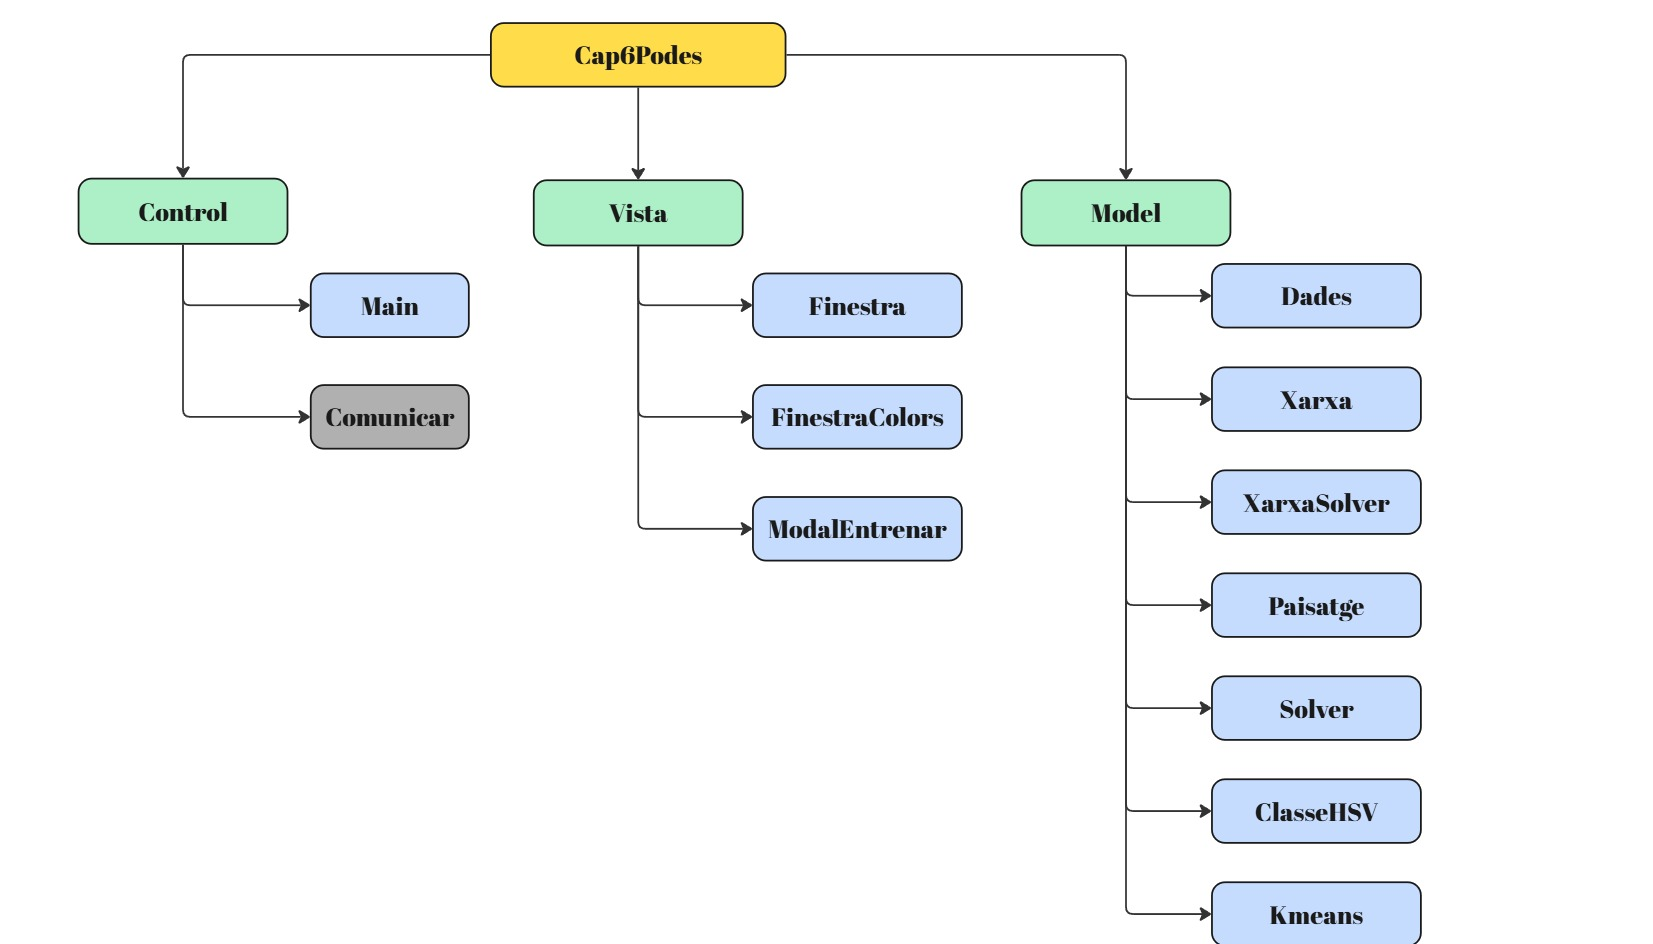
\includegraphics[width=0.45\textwidth]{png/estructure.jpg}
    \caption{Estructura del programa}
    \label{fig:enter-label}
\end{figure}
\subsection{Implementació del classificador HVS}
El classificador HVS s’implementa a la classe \texttt{ClassHSV}, que realitza els passos següents:
\begin{enumerate}
  \item Obté la imatge de \texttt{Dades} i determina l’amplada $W$ i l’alçada $H$.
  \item Calcula el nombre de mostres $n = \min(\texttt{samples}, W\times H)$.
  \item Per cada mostra:
    \begin{itemize}
      \item Tria aleatòriament un píxel $(x,y)$.
      \item Llegeix el color RGB i el converteix a HSV.
      \item Decideix la categoria (\emph{Verd}, \emph{Blau} o \emph{Altres}) comparant $(H,S,V)$ amb els rangs definits.
      \item Incrementa el comptador corresponent i, si és \emph{Verd}, acumula la saturació per al càlcul posterior.
    \end{itemize}
  \item Calcula les proporcions $p_\text{verd}$, $p_\text{blau}$, $p_\text{altres}$ dividint per $n$.
  \item Determina la categoria dominant i, en cas de \emph{Verd}, revisa la saturació mitjana per diferenciar \emph{bosc} vs. \emph{selva}.
  \item Emmagatzema a \texttt{Dades} els mapes de percentatges, marges d’error i l’etiqueta final.
\end{enumerate}

\begin{lstlisting}[language = Java, breaklines = true]
// Excerpt de ClassHSV.classificar(...)
BufferedImage img = dades.getImatge();
int w = img.getWidth(), h = img.getHeight();
int n = Math.min(samples, w*h);
Random rnd = new Random();
int cntV=0, cntB=0, cntO=0;
float satVSum = 0f;

for(int i=0; i<n; i++){
    int x = rnd.nextInt(w), y = rnd.nextInt(h);
    int rgb = img.getRGB(x,y);
    float[] hsv = Color.RGBtoHSB((rgb>>16)&0xFF,(rgb>>8)&0xFF,rgb&0xFF,null);
    float H = hsv[0]*360, S = hsv[1], V = hsv[2];
    if(isVerd(H,S,V)){ cntV++; satVSum += S; }
    else if(isBlau(H,S,V)) cntB++;
    else cntO++;
}
// calcul de proporcions, marges i decisio final...
\end{lstlisting}

\subsection{Modelització dels rangs HSV}
Per categoritzar cada píxel s’han definit els llindars següents:
\begin{itemize}
  \item \textbf{Verd (vegetació)}:
    \[
      60^\circ \le H < 170^\circ,\quad S > 0.20,\quad V > 0.20
    \]
  \item \textbf{Blau (cel/mar)}:
    \[
      180^\circ \le H < 260^\circ,\quad S > 0.15,\quad V > 0.20
    \]
  \item \textbf{Altres (terra, troncs, roques)}:
    \[
      \text{la resta de combinacions de }(H,S,V)
    \]
\end{itemize}
Aquests rangs s’han escollit basant-se en l’estudi de mostres representatives de cada paisatge, garantint un bon compromís entre robustesa i simplicitat.

\subsection{Xarxa neuronal}
La xarxa neuronal que implementa \texttt{Xarxa.java} realitza les següents funcionalitats
\begin{itemize}
    \item Configurar el nombre d'entrades, forma de les capes ocultes, i sortides. A més d'ajustar aleatòriament els pesos de les connexions.
    \item Predir el resultat d'una entrada.
    \item Entrenar la xarxa neuronal, amb backpropagation\cite{backpropagation} segons un número d'èpoques, o fins que convergeix.
    \item Amb \texttt{Serializable} es pot guardar l'estat de la xarxa una vegada entrenada.
\end{itemize}
Però la xarxa treballa amb nombres decimals, no amb imatges, per tant fa falta la classe \texttt{XarxaSolver} que s'encarregarà de llegir la imatge, extreure els percentatges de colors, i entrenar la xarxa.

\subsection{Utilitzar la xarxa}
La classe \texttt{XarxaSolver.java}, que implementa \texttt{Solver}, s'encarrega de la comunicació amb la xarxa. Aquesta comunicació és fonamental per passar les dades cap a la xarxa, entrenar-la amb les dades de prova i transmetre a la resta del programa el resultat d'una classificació.  
La xarxa utilitzada és una de 10 entrades (tantes com colors), amb dues capes ocultes de 8 i 6 neurones respectivament, i 3 sortides (una per paisatge).  
Amb \texttt{generarEntrada()}, es crea una entrada —els percentatges de cada color— a partir d'una imatge:

\begin{lstlisting}
public double[] generarEntrada(BufferedImage img){
    int pixels = img.getWidth() * img.getHeight();

    double[] entrada = new double[Colors.values().length];
    int[] colorIndex = new int[Colors.values().length];
    List<float[]> colors = new ArrayList<>();
    for (int i = 0; i < img.getHeight(); i++) {
        for (int k = 0; k < img.getWidth(); k++) {
            colorIndex[getColorIndex(img.getRGB(k, i))]++;
            colors.add(hsv);
        }
    }
    for (int i = 0; i < colorIndex.length; i++) {
        entrada[i] = colorIndex[i] / (double) pixels;
    }
    return entrada;
}
\end{lstlisting}
Per obtenir el color, es converteix el color a HSV i, segons el rang (\textit{hue}) i la seva brillantor (\textit{value}), se selecciona un color.
\begin{lstlisting}
public int getColorIndex(int color){
    Color c = new Color(color, false);
    float[] HSB = Color.RGBtoHSB(c.getRed(), c.getGreen(), c.getBlue(), null);
    float H = HSB[0] * 360;
    float S = HSB[1] * 100;
    float B = HSB[2] * 100;
    float A = c.getAlpha();

    if(A < 150){
        return Colors.BLANC.ordinal();
    }
    if(B < 15){
        return Colors.NEGRE.ordinal();
    }
    if(S < 17){
        return Colors.BLANC.ordinal();
    }

    if(H >= 75 && H < 155){
        if(B < 60){
            return Colors.VERD_OBSCUR.ordinal();
        }
        return Colors.VERD_CLAR.ordinal();
    }
    if(H >= 155 && H < 260){
        return Colors.BLAU.ordinal();
    }
    // continua...
\end{lstlisting}
\subsection{Càlcul del marge d’error}
Per cada categoria amb proporció $p_i$ sobre $n$ mostres, el marge d’error al 95\,\% es calcula com:
\[
  \mathrm{moe}_i \;=\; z \,\sqrt{\frac{p_i(1-p_i)}{n}}
  \quad\text{on }z = 1.96.
\]
Per garantir un marge màxim $\varepsilon$, la mida de mostra mínima $n$ s’estima amb:
\[
  n \;=\;\left\lceil \frac{z^2\,p(1-p)}{\varepsilon^2} \right\rceil,
\]
assumint $p=0.5$ per al cas més conservador. Aquests càlculs permeten quantificar la confiança de la classificació per a cada categoria.
\subsection{Kmeans}

La classe \texttt{Kmeans.java} implementa l'algorisme clàssic d'agrupació \emph{K}-Means\cite{KMeans}. El seu constructor principal rep dos paràmetres: \(K\), que especifica el nombre de \emph{clústers} a crear, i \texttt{maxIterations}, que determina el nombre màxim d'iteracions permeses.\newline

Les passes principals de l'algorisme són les següents:
\begin{itemize}
    \item Triar \(K\) centroïdes inicials de manera aleatòria.
    \item Assignar cada color de la llista \texttt{colors} al centroide més proper, utilitzant la distància definida en l'espai \emph{HSV}.
    \item Recalcular els nous centroïdes a partir de la mitjana dels colors assignats.
\end{itemize}

L'algorisme utilitza una variable booleana, \textbf{changed}, que permet detectar si hi ha hagut canvis en l'assignació dels colors. Si en una iteració no es produeixen canvis, és a dir l'algorisme ha convergit, el càlcul finalitza abans d'arribar al nombre màxim d'iteracions definit per \texttt{maxIterations}, reduint així el temps d'execució de l'algorisme.\newline

Al final, es calcula el percentatge de cada \emph{clúster} trobat, i es guarden tant els centroïdes —considerats com els colors dominants— com els percentatges associats, a la classe \texttt{Dades.java}.\newline

La distància entre dos colors en l'espai \emph{HSV} ve donada per la següent fórmula:

\[
\begin{aligned}
dh &= \min\Big(\big| \tfrac{H_1}{360} - \tfrac{H_2}{360} \big|,\, 
           1 - \big| \tfrac{H_1}{360} - \tfrac{H_2}{360} \big| \Big) \,, \\
ds &= |S_1 - S_2| \,, \\
dv &= |V_1 - V_2| \,. 
\end{aligned}
\]

Així, la distància total en l’espai \emph{HSV} queda definida com:
\[
d_\mathit{HSV}(c_1, c_2) = \sqrt{dh^2 + ds^2 + dv^2}\,.
\]


En aquest context, la component \(H\) (to) es normalitza per representar-la en l'interval \([0,1]\), ja que és una variable angular definida en \([0,360°]\). Les components \(S\) (saturació) i \(V\) (valor), en canvi, ja es troben normalitzades en l'interval \([0,1]\).


\begin{lstlisting}[language = Java, breaklines = true]
private void kMeans() {
    Random rnd = new Random();
    colors = dades.getColors();
   //triar els centroids de forma aleatoria
    centroids = new ArrayList<>();
    for (int i = 0; i < K; i++) {
        float[] randomColor = colors.get(rnd.nextInt(colors.size()));            centroids.add(randomColor);
    }
    //assignar cada color a un cluster
    int[] assignments = new int[colors.size()];
    for (int iter = 0; iter < maxIterations; iter++) {
        boolean changed = false;
        for (int i = 0; i < colors.size(); i++) {
            float[] color = colors.get(i);
            int closest = -1;
            double minDist = Double.MAX_VALUE;
            for (int j = 0; j < centroids.size(); j++) {
                float[] centroid = centroids.get(j);
                double dist = distanceHSV(color, centroid);
                if (dist < minDist) {
                    minDist = dist;
                    closest = j;
                }
            }
            if (assignments[i] != closest) {
                assignments[i] = closest;
                changed = true;
            }
        }
        //convergencia
        if (!changed) break;
        //promig dels centroids
        float[][] newCentroids = new float[K][3];
        int[] counts = new int[K];
        for (int i = 0; i < colors.size(); i++) {
            int cluster = assignments[i];
            float[] color = colors.get(i);
            for (int k = 0; k < 3; k++) {
                newCentroids[cluster][k] += color[k];
            }
            counts[cluster]++;
        }
        for (int j = 0; j < K; j++) {
            if (counts[j] > 0) {
                for (int k = 0; k < 3; k++) {
                    newCentroids[j][k] /= counts[j];
                }
                centroids.set(j, newCentroids[j]);
            }
        }
    }
  clusterCounts = new int[K];
    for (int cluster : assignments) {
        clusterCounts[cluster]++;
    }
}

\end{lstlisting}
\subsection{Gestió de concurrència} 
Com es costum en les nostres pràctiques, la interfície s'executa en el seu propi thread, a més, cada execució d'un \texttt{Solver} es fa sobre un thread dins un \texttt{ExecutorService}.
A més, es controla l'aturada controlada dins els solvers amb la funció aturar de \texttt{Comunicar}.

\subsection{Visualització i interacció amb l'usuari}
La finestra principal ofereix les següents funcionalitats: permet carregar imatges i visualitzar-les directament, classificar-les utilitzant una xarxa neuronal o bé a partir de la distribució dels colors en l'espai \emph{HSV}, entrenar( i aturar) una xarxa neuronal, i finalment, aturar l'execució del procés principal.


\begin{figure}[H]
    \centering
    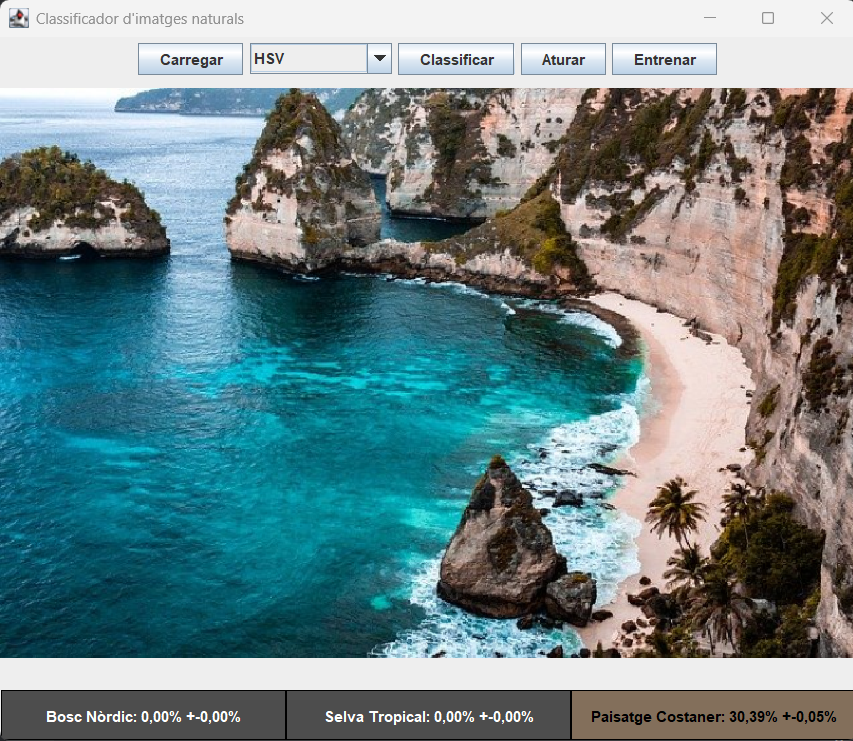
\includegraphics[width=0.45\textwidth]{png/finestra.png}
    \caption{Finestra principal}
    \label{fig:enter-label}
\end{figure}
A més, en executar el programa es crea una segona finestra, encarregada de representar els colors dominants de la imatge. Mitjançant l'algorisme de \emph{K}-Means, aquesta finestra rep com a paràmetres el nombre de colors a determinar (és a dir, el nombre de \emph{clústers}) i el nombre màxim d'iteracions per al càlcul. Finalment, mostra els colors dominants obtinguts.

\begin{figure}[H]
    \centering
    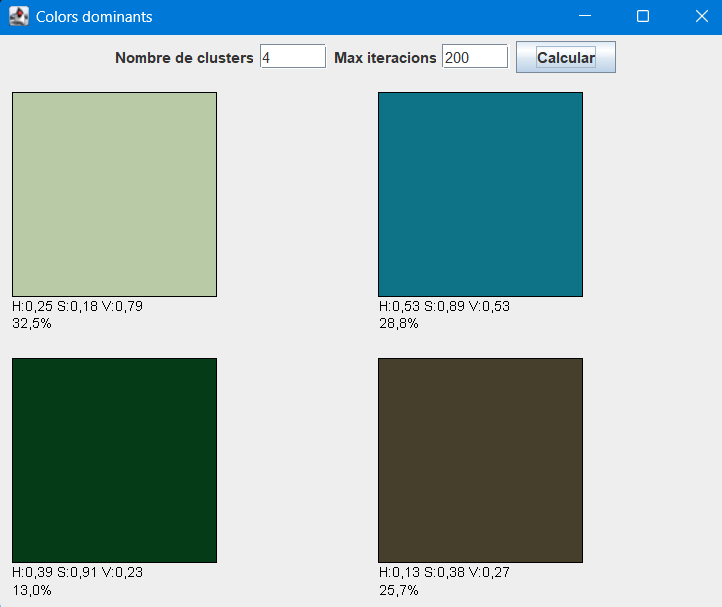
\includegraphics[width=0.45\textwidth]{png/colors.png}
    \caption{Finestra de colors dominants}
    \label{fig:enter-label}
\end{figure}

\subsection{Flux de control i comunicació}

El flux de control i la comunicació entre components segueixen fidelment el patró Model–Vista–Controlador (MVC). La classe \texttt{Main} actua com a controlador principal, gestionant els esdeveniments de la interfície gràfica i delegant les operacions al model de manera asincrònica. Per tal de garantir una arquitectura desacoblada i modular, s'ha dissenyat una interfície pròpia anomenada \texttt{Comunicar}, que defineix un conjunt de mètodes estàndard per a la comunicació entre la vista, el controlador i els solvers del model.

\paragraph{Interfície \texttt{Comunicar}}

Aquesta interfície inclou operacions com ara:

\begin{itemize}
  \item \texttt{carregarImatge(String ruta)}: permet que la vista sol·liciti la càrrega d'una imatge al model.
  \item \texttt{classificarHSV()} i \texttt{classificarXarxa()}: activen els processos de classificació corresponents.
  \item \texttt{comunicar(String msg)}: canal de comunicació genèric per enviar missatges i estats entre components.
  \item \texttt{actualitzarFinestra()}: utilitzat per actualitzar la vista quan hi ha canvis en les dades.
\end{itemize}

Aquesta interfície és implementada pel controlador \texttt{Main}, i és passada als components que en necessiten accés, com ara la classe \texttt{Finestra} i els diferents solvers (\texttt{ClassHSV}, \texttt{XarxaSolver}).

\paragraph{Controlador i gestió de tasques}

Per garantir una execució fluida i no bloquejant, el controlador empra un \texttt{ExecutorService} amb un únic fil d'execució:

\begin{lstlisting}[language=Java]
private final ExecutorService executor = Executors.newSingleThreadExecutor();
\end{lstlisting}

Això permet executar els processos de classificació de manera independent del fil d'UI, mantenint la responsivitat de la interfície. La crida a un solver es fa així:

\begin{lstlisting}[language=Java]
@Override
public void classificarHSV() {
    Solver solver = new ClassHSV();
    executor.submit(solver);
}
\end{lstlisting}

Cada solver (com \texttt{ClassHSV} i \texttt{XarxaSolver}) implementa la interfície \texttt{Runnable} i, un cop finalitzat el seu procés, pot comunicar-se amb el controlador a través del mètode \texttt{comunicar}.

\paragraph{Patró \emph{Singleton} i compartició de dades}

La classe \texttt{Main} s’implementa com un \emph{singleton}, de manera que
l’únic punt d’accés global al controlador és el mètode
\texttt{getInstance()}.  
Això permet:

\begin{enumerate}
  \item Compartir el mateix objecte \texttt{Dades} entre tots els components:
        el model és creat una sola vegada dins \texttt{Main} i recuperat des
        de qualsevol lloc amb:
\begin{lstlisting}[language=Java]
Dades dades = Main.getInstance().getDades();
\end{lstlisting}

  \item Facilitar les crides de la vista cap al controlador sense afegir
        dependències dures.  A la classe \texttt{Finestra} s’obté la referència
        al controlador així:

\begin{lstlisting}[language=Java]
Comunicar controlador = Main.getInstance();
controlador.carregarImatge(rutaFitxer);
controlador.classificarHSV();   // o classificarXarxa()
\end{lstlisting}

  \item Garantir coherència de l’estat: com que tots els \texttt{Solver} i la
        vista treballen sobre la mateixa instància de \texttt{Dades}, no hi ha
        duplicació d’informació.  A més, qualsevol modificació es fa sempre
        dins el fil gestionat per l’\texttt{ExecutorService}; la vista només
        llegeix els resultats mitjançant \texttt{SwingUtilities.invokeLater},
        evitant condicions de carrera.
\end{enumerate}

D’aquesta manera, el \emph{singleton} no trenca la separació de capes sinó que
serveix com a mecanisme de registre centralitzat perquè tots els actors
(MVC + \texttt{Solver}) comparteixin l’estat i es comuniquin mitjançant la
interfície \texttt{Comunicar}.


\paragraph{Desacoblament i comunicació estructurada}

Aquest enfocament modular permet que el model i la vista no es coneguin directament entre ells. El model, encapsulat en classes com \texttt{ClassHSV} i \texttt{Dades}, pot operar de manera independent i només comunica resultats a través del controlador. \newline
La vista, representada per la classe \texttt{Finestra}, també opera exclusivament mitjançant la interfície \texttt{Comunicar}, invocant mètodes sense dependre de la implementació específica del model.\newline

Aquesta arquitectura ofereix una gran flexibilitat i facilita la integració de nous classificadors (com el basat en xarxa neuronal), ja que aquests només necessiten accedir a les dades i notificar el controlador de l'estat de l'execució. Alhora, permet una gestió eficaç d'errors i estats mitjançant missatges textuals controlats centralment al \texttt{Main}.


\subsection{Decisions de disseny i extres implementats}
Pel que fa a l'algorisme de K-Means, el sistema de color \emph{HSV} (matís, saturació i valor) és preferit al model \emph{RGB} per a la segmentació de colors en imatges, ja que separa la informació del color de la informació de la il·luminació. Mentre que el model \emph{RGB} barreja la intensitat de la llum amb els components de color, el model \emph{HSV} aïlla el matís i la saturació — que representen el color pur — de la component de valor, que correspon al brillantor o intensitat lumínica. Aquesta separació fa que la segmentació basada en \emph{HSV} sigui més robusta davant canvis d'il·luminació, ombres o reflexos. A més, el matís té una interpretació més intuïtiva i directa amb els colors percebuts, permetent definir rangs més clars per identificar colors específics. Per tant, \emph{HSV} facilita la delimitació i classificació de regions en una imatge segons el seu color, millorant la precisió i consistència del procés de segmentació \cite{colorSegmentation2018} \cite{stackOverflowKMeans}.

També, una de les funcionalitats extra que s'han implementat, i com s'ha detallat prèviament en aquest document, és l'ús d'una xarxa neuronal per a la predicció del tipus dels paisatges.


\section{Resultats i Comparació} 
En aquesta secció es posa a prova el funcionament dels classificadors desenvolupats. El conjunt de dades utilitzat està format per imatges de paisatges prèviament etiquetades de manera correcta, les quals es troben emmagatzemades a la carpeta \textit{res}. L'obtenció dels resultats es basa en l'execució individual de cadascun dels classificadors sobre aquestes imatges, amb l'objectiu d'avaluar-ne la precisió i la robustesa.

\begin{table}[H]
\centering
\caption{Classificació de paisatges usant el mètode probabilístic}
\label{tab:clasificacion}
\begin{tabular}{|c|c|c|c|}
\hline
\textbf{Probabilístic} & \textbf{Bosc Nòrdic} & \textbf{Selva Tropical} & \textbf{Paisatge Costaner} \\
\hline
bosc\_0  & 3,64 & 0,00 & 17,14 \\
bosc\_1  & 0,002 & 0,00 & 0,00 \\
costa\_0 & 8,57 & 0,00 & 54,81 \\
costa\_1 & 5,71 & 0,52 & 23,38 \\
selva\_0 & 60,26 & 9,35 & 0,00 \\
selva\_1 & 33,77 & 18,70 & 0,26 \\
\hline
\end{tabular}
\end{table}


\begin{table}[H]
\centering
\caption{Classificació de paisatges usant la xarxa neuronal}
\label{tab:xarxa}
\begin{tabular}{|c|c|c|c|}
\hline
\textbf{Xarxa} & \textbf{Bosc Nòrdic} & \textbf{Selva Tropical} & \textbf{Paisatge Costaner} \\
\hline
bosc\_0  & 99,99 & 0     & 0,0  \\
bosc\_1  & 99,99 & 0     & 0,01  \\
costa\_0 & 0     & 1,76  & 99,99  \\
costa\_1 & 0,07  & 1,14  & 99,81 \\
selva\_0 & 0     & 99,94 & 0,02  \\
selva\_1 & 0     & 99,93 & 0,02  \\
\hline
\end{tabular}
\end{table}

Els resultats obtinguts es poden representar de manera visual mitjançant un gràfic de barres, que permet comparar fàcilment el rendiment dels diferents classificadors.
\begin{figure}[H]
    \centering
    \includegraphics[width=0.45\textwidth]{png/Resultats del classificador probabilístic.png}
    \caption{Resultats del classificador probabilístic}
    \label{fig:enter-label}
\end{figure}

\begin{figure}[H]
    \centering
    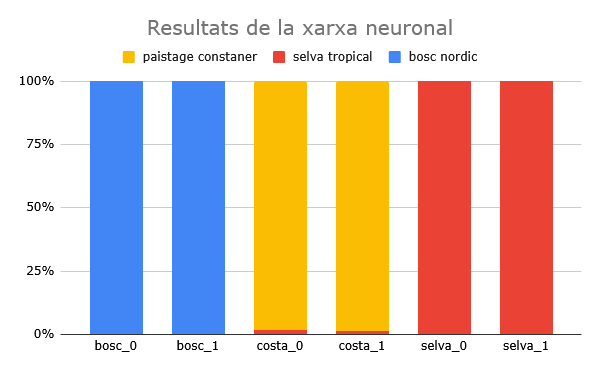
\includegraphics[width=0.45\textwidth]{png/Resultats de la xarxa neuronal.png}
    \caption{Resultats de la xarxa neuronal}
    \label{fig:enter-label}
\end{figure}

Els resultats permeten extreure una conclusió clara sobre l’eficàcia de cada classificador: la xarxa neuronal supera el classificador probabilístic. Amb un percentatge d'encert del \(100\%\), la xarxa ha etiquetat correctament els cinc paisatges, amb una precisió superior al \(90\%\) en cadascun d’aquests casos. En canvi, el classificador probabilístic només ha identificat correctament dos (el percentatge per al bosc\_1 és bastant petit)  dels cinc paisatges, aconseguint així un percentatge d’encert del \(40\%\).\newline

El rendiment modest del classificador probabilístic es pot atribuir principalment a dues limitacions clau. En primer lloc, els rangs de valors de to (\(H\)), saturació (\(S\)) i valor (\(V\)) assignats a cada paisatge poden no adaptar-se bé a la variabilitat cromàtica de totes les imatges. Sovint, els colors representatius de diferents paisatges presenten solapaments o es troben molt pròxims dins l'espai de color, la qual cosa dificulta una separació clara entre classes. \newline
En segon lloc, el procés de mostreig es basa en la selecció aleatòria de píxels de tota la imatge, sense tenir en compte la seva rellevància contextual ni la seva distribució espacial. Això pot portar a resultats poc representatius, especialment en imatges amb regions mixtes o amb presència de fons que no aporten informació útil per a la classificació.

\section{Conclusions} 
Aquesta pràctica ha resultat interessant, sobretot perquè tracta un aspecte ja vist durant la carrera i clau en el nostre itinerari: el problema de classificació d’imatges.  
S’ha abordat aquest repte amb dos enfocaments diferents: l’estudi de la distribució dels colors dominants en els paisatges per determinar rangs importants que permeten, mitjançant un mètode probabilístic, predir la classificació d’un paisatge donat; i, en segon lloc, l’entrenament d’una petita xarxa neuronal amb un conjunt de dades per aprendre a classificar les imatges.  
La xarxa neuronal s’entrena mitjançant l’algorisme de retropropagació d’errors (backpropagation), que ajusta iterativament els pesos de la xarxa per minimitzar l’error entre la predicció i la classificació esperada, fins a aconseguir una bona precisió o un nombre màxim d’iteracions.\newline

L'ús de l'algorisme K-Means va resultar útil per visualitzar els \(K\) colors dominants, tot i que no és del tot precís, ja que els centroides s'inicialitzen de manera aleatòria. \newline

Pel que fa a la distribució de tasques, en aquesta pràctica gairebé tothom ha participat en totes les fases. El model s'ha desenvolupat entre tres persones, la interfície gràfica entre dues, el controlador entre tres altres, i la redacció de la memòria ha estat una feina col·lectiva.


\bibliographystyle{IEEEtran}
\begin{thebibliography}{1}
\bibitem{KMeans}
Wikipedia, “K-means clustering,” \url{https://en.wikipedia.org/wiki/K-means_clustering}. Consultat el juny de 2025.

\bibitem{hammersley1964} J.~M. Hammersley i D.~C. Handscomb, \emph{Monte-Carlo-Methods}, Chapman \& Hall, 1964.
\bibitem{stackexchangeHSVtoRGB}
Stack Exchange, “Convert HSV to RGB colors,” \url{https://cs.stackexchange.com/questions/64549/convert-hsv-to-rgb-colors}. Consultat el juny de 2025.

\bibitem{smith1978} G.~Smith, “Color Gamut Transform Pairs,” \emph{Proc. Society for Information Display}, 1978.
\bibitem{gamma1994} E.~Gamma, R.~Helm, R.~Johnson i J.~Vlissides, \emph{Design Patterns: Elements of Reusable Object-Oriented Software}, Addison-Wesley, 1994.
\bibitem{colorSegmentation2018}
S. Kumari, R. K. Tripathi i P. K. Singh, \emph{Color Image Segmentation using Automated K-Means Clustering with RGB and HSV Color Spaces}, ResearchGate, 2018. Disponible a: \url{https://www.researchgate.net/publication/328612893_Color_Image_Segmentation_using_Automated_K-Means_Clustering_with_RGB_and_HSV_Color_Spaces}.

\bibitem{ann} Roheen Qamar, Baqar Ali Zardar \emph{Artificial Neural Networks: An Overview} \url{https://www.researchgate.net/publication/373700317_Artificial_Neural_Networks_An_Overview}
\bibitem{backpropagation} David E.Rumelhart, Geoffrey E. Hinton, Ronald J. Williams, \emph{Learning representations by back-propagating errors} \url{https://www.iro.umontreal.ca/~vincentp/ift3395/lectures/backprop_old.pdf}

\bibitem{stackOverflowKMeans}
Stack Overflow, \emph{K-means clustering on RGB or HSV scale}, 2015. Disponible a: \url{https://stackoverflow.com/questions/32447729/k-means-clustering-on-rgb-or-hsv-scale}.

\bibitem{gafter1999} J.~Gafter, “Swing Architecture and Concepts,” JavaOne Conference, 1999.
\end{thebibliography}

\end{document}


